
%(BEGIN_QUESTION)
% Copyright 2011, Tony R. Kuphaldt, released under the Creative Commons Attribution License (v 1.0)
% This means you may do almost anything with this work of mine, so long as you give me proper credit

This control system controls ``waste'' fuel gas header pressure by venting gas into the burner.  It also limits the flow of ``waste'' gas when excessive, through the use of an override control strategy.  The red-colored, italicized numbers indicate ``live'' signal values at one point in time:

$$\includegraphics[width=15.5cm]{i02460x01.eps}$$

Answer the following questions, based on what you see in this diagram:

\begin{itemize}
\item{} Which waste gas controller is in control right now, and which one is being overridden?
\vskip 10pt
\item{} Does there appear to be a surplus of waste fuel gas available to this system right now, or a deficiency?
\vskip 10pt
\item{} Identify at least two changes that could take place in this process to switch control from one waste gas controller to the other.
\end{itemize}

\underbar{file i02460}
%(END_QUESTION)





%(BEGIN_ANSWER)

\noindent
{\bf Partial answer:}

\vskip 10pt

The PC is currently in control, overriding the FC.

%(END_ANSWER)





%(BEGIN_NOTES)

Right now there is a deficit of waste gas, which is why pressure control is overriding flow control: the valve needs to pinch down in order to build the waste gas header pressure up to setpoint.

\vskip 10pt

Here are some changes which could cause control to switch back to flow (from pressure):

\begin{itemize}
\item{} More waste gas becomes available to the system
\item{} The firing rate demand signal decreases below 36.9\%
\item{} The minimum waste fuel ratio setpoint decreases below 44.8\%
\end{itemize}

%INDEX% Control, strategies: override control
%INDEX% Control, strategies: waste fuel flow control system
%INDEX% Process: combustion furnace

%(END_NOTES)


